

\tikzset{every picture/.style={line width=0.75pt}} %set default line width to 0.75pt        

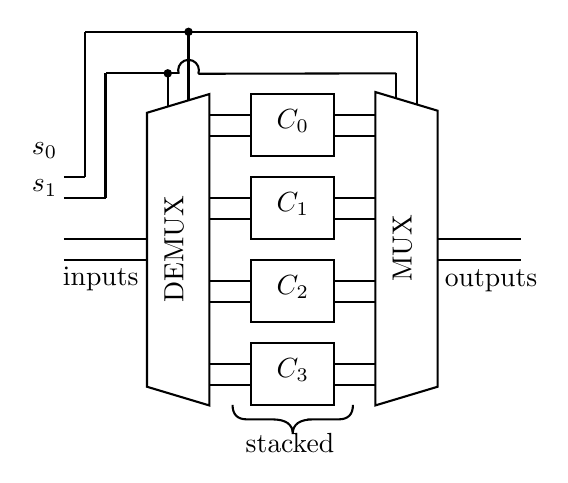
\begin{tikzpicture}[x=0.75pt,y=0.75pt,yscale=-1,xscale=1]
%uncomment if require: \path (0,300); %set diagram left start at 0, and has height of 300

%Shape: Rectangle [id:dp048587029840014395] 
\draw   (120,40) -- (160,40) -- (160,70) -- (120,70) -- cycle ;
%Shape: Rectangle [id:dp5776713339273196] 
\draw   (120,80) -- (160,80) -- (160,110) -- (120,110) -- cycle ;
%Shape: Rectangle [id:dp6797954191886235] 
\draw   (120,120) -- (160,120) -- (160,150) -- (120,150) -- cycle ;
%Shape: Rectangle [id:dp13612273639531247] 
\draw   (120,160) -- (160,160) -- (160,190) -- (120,190) -- cycle ;
%Shape: Trapezoid [id:dp8246309150363402] 
\draw   (100,190) -- (70,181) -- (70,49) -- (100,40) -- cycle ;
%Straight Lines [id:da7525185807979242] 
\draw    (100,60) -- (120,60) ;
%Straight Lines [id:da31461604940557963] 
\draw    (100,50) -- (120,50) ;
%Straight Lines [id:da25486541008995456] 
\draw    (100,100) -- (120,100) ;
%Straight Lines [id:da0077951778335063615] 
\draw    (100,90) -- (120,90) ;
%Straight Lines [id:da2905976026522047] 
\draw    (100,140) -- (120,140) ;
%Straight Lines [id:da7452387399270697] 
\draw    (100,130) -- (120,130) ;
%Straight Lines [id:da0007664179468291898] 
\draw    (100,180) -- (120,180) ;
%Straight Lines [id:da10206153239828308] 
\draw    (100,170) -- (120,170) ;
%Straight Lines [id:da762851249257401] 
\draw    (160,60) -- (180,60) ;
%Straight Lines [id:da7906149158989283] 
\draw    (160,50) -- (180,50) ;
%Straight Lines [id:da7502678160942512] 
\draw    (160,100) -- (180,100) ;
%Straight Lines [id:da9029629905302936] 
\draw    (160,90) -- (180,90) ;
%Straight Lines [id:da3474710624597941] 
\draw    (160,140) -- (180,140) ;
%Straight Lines [id:da15085166543146156] 
\draw    (160,130) -- (180,130) ;
%Straight Lines [id:da33183615362638585] 
\draw    (160,180) -- (180,180) ;
%Straight Lines [id:da3689964414613789] 
\draw    (160,170) -- (180,170) ;
%Shape: Trapezoid [id:dp3485611043917566] 
\draw   (180,39) -- (210,48) -- (210,181) -- (180,190) -- cycle ;
%Straight Lines [id:da03742821351482728] 
\draw    (30,120) -- (70,120) ;
%Straight Lines [id:da7640218221254925] 
\draw    (30,110) -- (70,110) ;
%Straight Lines [id:da956984886166125] 
\draw    (210,120) -- (250,120) ;
%Straight Lines [id:da3748285907762332] 
\draw    (210,110) -- (250,110) ;
%Straight Lines [id:da9714588986108855] 
\draw    (30,90) -- (50,90) ;
%Straight Lines [id:da8529976703877445] 
\draw    (30,80) -- (40,80) ;
%Straight Lines [id:da30690121561733863] 
\draw    (50,30) -- (50,90) ;
%Straight Lines [id:da15914818103441886] 
\draw    (85,30) -- (50,30) ;
%Straight Lines [id:da11238885987153702] 
\draw    (80,30) -- (80,46) ;
%Straight Lines [id:da3144505075089207] 
\draw    (40,10) -- (40,80) ;
%Straight Lines [id:da8817997683520893] 
\draw    (200,10) -- (40,10) ;
%Straight Lines [id:da4268960799866157] 
\draw    (90,43) -- (90,10) ;
%Shape: Arc [id:dp9375967782263986] 
\draw  [draw opacity=0] (85.3,30.21) .. controls (85.11,29.68) and (85,29.1) .. (85,28.5) .. controls (85,25.74) and (87.24,23.5) .. (90,23.5) .. controls (92.76,23.5) and (95,25.74) .. (95,28.5) .. controls (95,29.1) and (94.89,29.68) .. (94.7,30.21) -- (90,28.5) -- cycle ; \draw   (85.3,30.21) .. controls (85.11,29.68) and (85,29.1) .. (85,28.5) .. controls (85,25.74) and (87.24,23.5) .. (90,23.5) .. controls (92.76,23.5) and (95,25.74) .. (95,28.5) .. controls (95,29.1) and (94.89,29.68) .. (94.7,30.21) ;
%Straight Lines [id:da20395268049972604] 
\draw    (190,30) -- (94.7,30.21) ;
%Straight Lines [id:da9984121684679509] 
\draw    (190,42) -- (190,30) ;
%Straight Lines [id:da8655654304921162] 
\draw    (200,45) -- (200,10) ;
%Shape: Circle [id:dp15675574970767925] 
\draw  [fill={rgb, 255:red, 0; green, 0; blue, 0 }  ,fill opacity=1 ] (78.5,30) .. controls (78.5,29.17) and (79.17,28.5) .. (80,28.5) .. controls (80.83,28.5) and (81.5,29.17) .. (81.5,30) .. controls (81.5,30.83) and (80.83,31.5) .. (80,31.5) .. controls (79.17,31.5) and (78.5,30.83) .. (78.5,30) -- cycle ;
%Shape: Circle [id:dp007756137419556719] 
\draw  [fill={rgb, 255:red, 0; green, 0; blue, 0 }  ,fill opacity=1 ] (88.5,10) .. controls (88.5,9.17) and (89.17,8.5) .. (90,8.5) .. controls (90.83,8.5) and (91.5,9.17) .. (91.5,10) .. controls (91.5,10.83) and (90.83,11.5) .. (90,11.5) .. controls (89.17,11.5) and (88.5,10.83) .. (88.5,10) -- cycle ;
%Shape: Brace [id:dp3366641720684751] 
\draw   (111.21,189.72) .. controls (111.21,194.39) and (113.54,196.72) .. (118.21,196.72) -- (130.21,196.72) .. controls (136.88,196.72) and (140.21,199.05) .. (140.21,203.72) .. controls (140.21,199.05) and (143.54,196.72) .. (150.21,196.72)(147.21,196.72) -- (162.21,196.72) .. controls (166.88,196.72) and (169.21,194.39) .. (169.21,189.72) ;

% Text Node
\draw (131,45.93) node [anchor=north west][inner sep=0.75pt]   [align=left] {$\displaystyle C_{0}$};
% Text Node
\draw (131,85.93) node [anchor=north west][inner sep=0.75pt]   [align=left] {$\displaystyle C_{1}$};
% Text Node
\draw (131,125.93) node [anchor=north west][inner sep=0.75pt]   [align=left] {$\displaystyle C_{2}$};
% Text Node
\draw (131,165.93) node [anchor=north west][inner sep=0.75pt]   [align=left] {$\displaystyle C_{3}$};
% Text Node
\draw (13,61.93) node [anchor=north west][inner sep=0.75pt]   [align=left] {$\displaystyle s_{0}$};
% Text Node
\draw (13,79.93) node [anchor=north west][inner sep=0.75pt]   [align=left] {$\displaystyle s_{1}$};
% Text Node
\draw (76.93,142) node [anchor=north west][inner sep=0.75pt]  [rotate=-270] [align=left] {DEMUX};
% Text Node
\draw (186.93,132) node [anchor=north west][inner sep=0.75pt]  [rotate=-270] [align=left] {MUX};
% Text Node
\draw (28,121.93) node [anchor=north west][inner sep=0.75pt]   [align=left] {inputs};
% Text Node
\draw (212,122.93) node [anchor=north west][inner sep=0.75pt]   [align=left] {outputs};
% Text Node
\draw (116,201.93) node [anchor=north west][inner sep=0.75pt]   [align=left] {stacked};


\end{tikzpicture}

